A one-dimensional range tree is a binary search tree on one-dimensional 
point data. 
The point data of the tree is stored in the leaves. 
Each inner vertex stores the highest entry of its left subtree.
The version of a range tree implemented here is static, which means that 
after construction of the tree, no elements be inserted or deleted.
A $d$-dimensional range tree is a binary leaf search tree according to the 
first dimension of the $d$-dimensional point data, where each vertex contains 
a $(d-1)$-dimensional search tree of the points in the subtree (sublayer tree)
with respect to the second dimension.
See~\cite{bkos-cgaa-97} and~\cite{s-dasds-90} for more detailed information.

A $d$-dimensional range tree can be used to determine all
$d$-dimensional points that lie inside  a given $d$-dimensional
interval (\ccStyle{window\_query}).
\begin{ccTexOnly}
Figure~\ref{User:fig:range.eps} shows a two-dimensional range tree,
Figure~\ref{User:fig:d-range.eps} a $d$-dimensional one.
\end{ccTexOnly}
\begin{ccHtmlOnly}
The pictures below show a two-dimensional and a <span class="math">d</span>-dimensional
range tree.
\end{ccHtmlOnly}
\begin{ccTexOnly}
    \begin{figure}[htbp]
    \begin{minipage}{7cm}
    \begin{center}
    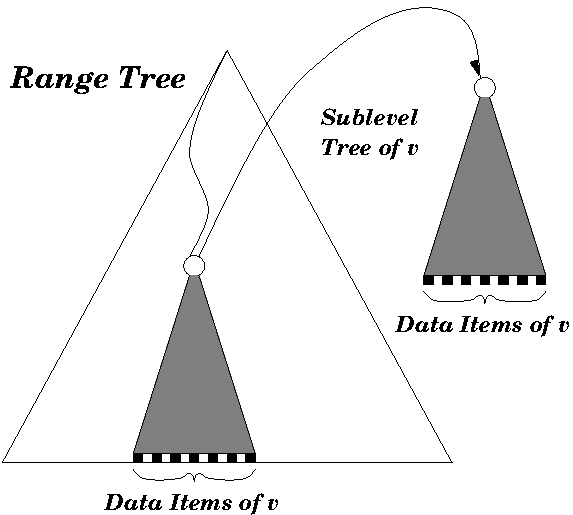
\includegraphics[width=7cm,clip]{SearchStructures/range2}
    \end{center}
    \caption{\label{User:fig:range.eps}A two-dimensional range tree. The
      tree is a binary search tree on the first dimension. Each
      sublayer tree of a vertex $v$ is a binary search tree on the second
      dimension. The data items in a sublayer tree of $v$ are
      all data items of the subtree of $v$.}
    \end{minipage}
    \hspace*{1em}
    \begin{minipage}{7cm}
    \begin{center}
    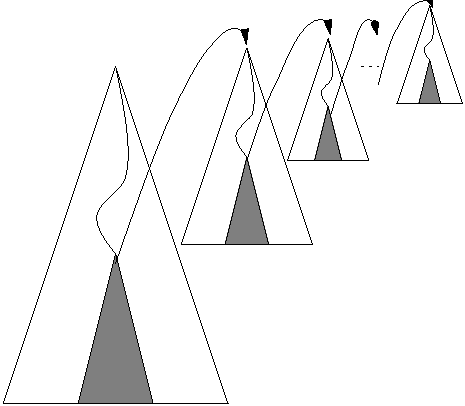
\includegraphics[width=7cm,clip]{SearchStructures/d-range}
    \end{center}
    \caption{\label{User:fig:d-range.eps}A d-dimensional range tree. For
      each layer of the tree, one
      sublayer tree is illustrated.}
    \vspace{2\baselineskip}
    %
    \end{minipage}
    \end{figure}
\end{ccTexOnly}

\begin{ccHtmlOnly}
    <!2><TABLE BORDER=0 CELLSPACING=2 CELLPADDING=0 WIDTH=650>
        <TR><TD ALIGN=LEFT VALIGN=TOP WIDTH=50% NOWRAP COLSPAN=2>
    <A NAME="User:fig:range.eps"><img border=0 src="./range2.gif" alt="A two-dimensional range tree"></A>
    </TD>
    <A NAME="User:fig:d-range.eps"><TD ALIGN=LEFT VALIGN=TOP WIDTH=50%><img border=0 src="./d-range.gif" alt="A d-dimensional range tree"></A>
      </TD></TR></TABLE>
        <!2><TABLE BORDER=0 CELLSPACING=2 CELLPADDING=0 WIDTH=650>
        <TR><TD ALIGN=LEFT VALIGN=TOP WIDTH=45%  COLSPAN=2>
    A two-dimensional range tree. The
      tree is a binary search tree on the first dimension. Each
      sublayer tree of a vertex <span class="math">v</span> is a binary search tree on the
second
      dimension. The data items in a sublayer tree of <span class="math">v</span> are
      all data items of the subtree of <span class="math">v</span>
 </TD><TD ALIGN=LEFT VALIGN=TOP WIDTH=50%>
A d-dimensional range tree. For
      each layer of the tree, one
      sublayer tree is illustrated.
 </TD></TR>
        </TABLE><!2>

\end{ccHtmlOnly}

%The tree can be built in  ${\cal O}(n\log^{d-1} n)$ time and
%needs  ${\cal O}(n\log^{d-1} n)$ space. The $d$-dimensional points that lie in the
%$d$-dimensional query interval can be reported in ${\cal O}(\log^dn+k)$ time,
%where $n$ is the total number of points and $k$ is the number of
%reported points. 

The tree can be built in  $O(n\log^{d-1} n)$ time and
needs  $O(n\log^{d-1} n)$ space. The $d$-dimensional points that lie in the
$d$-dimensional query interval can be reported in $O(\log^dn+k)$ time,
where $n$ is the total number of points and $k$ is the number of
reported points. 
